\chapter{Methodology}
\label{chapter_methodology}

In this chapter, we present the detailed formalism of Finite Difference Time Domain - Particle In Cell (FDTD/PIC) method in the Lorentz boosted coordinate system.
%
There are many small still very important considerations in order to obtain reliable results, which converge to the real values.
%
For example, the method for electron bunch generation, particle pusher algorithm and computational mesh truncation need particular attention.

\section{Finite Difference Time Domain (FDTD)}
\label{section FDTD}

FDTD is perhaps the first choice coming to mind for solving partial differential equations governing the dynamics of a system.
%
Despite its simple formulation and second order accuracy, there are certain features in this method like explicit time update and zero DC fields, which makes this method a superior choice compared to other algorithms \cite{taflove2000computational}.
%
FDTD samples the field in space and time at discrete sampling points and represents the partial derivatives with their discrete counterparts.
%
Subsequently, update equations are derived based on the governing differential equation.
%
Using these updating equations, a time marching algorithm is acquired which evaluates the unknown functions in the whole computational domain throughout the simulation time.
%
In the following, we start with the wave equation which is the governing partial differential equation for our electromagnetic problem.

\subsection{Wave Equation}
The physics of electromagnetic wave and its interaction with charged particles in free space is mathematically formulated through the well-known Maxwell's equations:
%
\begin{align}
\nabla \times \vec{E} &= -\frac{\displaystyle \partial \vec{B}}{\displaystyle \partial t} \\
\nabla \times \vec{B} &= \mu_0 \vec{J} + \mu_0 \varepsilon_{0} \frac{\displaystyle \partial \vec{E}}{\displaystyle \partial t} \\
\nabla \cdot \vec{E} &= -\frac{\displaystyle \rho}{\displaystyle \varepsilon_{0}} \\
\nabla \cdot \vec{B} &= 0
\end{align}
%
These equations in conjunction with the electric current equation $\vec{J}=\rho \vec{v}$ ($\vec{v}$ is the charge velocity) and the Lorentz force equation:
%
\begin{equation}
\label{LorentzForce}
\vec{F} = q(\vec{E} + \vec{v} \times \vec{B})
\end{equation}
%
are sufficient to describe wave-electron interaction in free space.
%
Moving free electrons introduce electric current which enters into the Maxwell's equations as the source.
%
Electric and magnetic fields derived from these equations are subsequently employed in the Lorentz force equation to determine the forces on the electrons, which in turn determine their motions.
%
As it is evident from the above equations, there are two unknown vectors ($\vec{E}$ and $\vec{B}$) to be evaluated, meaning that six unknown components should be extracted from the equations.
%
However, since these two vectors are interrelated and specially because there is no magnetic monopole in the nature ($\nabla \cdot \vec{B}=0 $), one can recast Maxwell's equations in a wave equation for the magnetic vector potential ($\vec{A}$) and a wave equation for the scalar electric potential ($\varphi$):
%
\begin{equation}
\label{WaveA}
{\vec{\nabla}}^{2}\vec{A} - \frac{1}{c^2} \frac{\displaystyle \partial^2}{\displaystyle \partial t^2}\vec{A} = -\mu_{0} \vec{J}
\end{equation}
%
\begin{equation}
\label{WaveF}
{\nabla}^{2}\varphi- \frac{1}{c^2} \frac{\displaystyle \partial^2 \varphi}{\displaystyle \partial t^2} = -\frac{\displaystyle \rho}{\displaystyle \varepsilon_{0}},
\end{equation}
%
where $c=1/\sqrt{\mu_0 \varepsilon_0}$ is the light velocity in vacuum.
%
In the derivation of above equations, the Lorentz gauge $\nabla \cdot \vec{A}=-\frac{1}{c^2}\frac{\partial \varphi}{\partial t}$ is used. %%
%
The original $\vec{E}$ and $\vec{B}$ vectors can be obtained from $\vec{A}$ and $\varphi$ as:
%
\begin{equation}
\label{BvsA}
\vec{B} = \nabla \times \vec{A}
\end{equation}
%
\begin{equation}
\label{EvsA}
\vec{E} = -\frac{\partial \vec{A}}{\partial t}-\nabla \varphi
\end{equation}
%
In addition to the above equations, the charge conservation law written as
%
\begin{equation}
\label{chargeLaw}
\nabla \cdot \vec{J} + \frac{\partial \rho}{\partial t} = 0,
\end{equation}
should not be violated in the employed computational algorithm.
%
This is the main motivation for seeking proper current deposition algorithms in the FDTD/PIC methods used for plasma simulations.
%
It is immediately observed that the equations (\ref{WaveA}), (\ref{WaveF}), (\ref{chargeLaw}) and the Lorentz gauge introduce an overdetermined system of equations.
%
In other words, once a current deposition is implemented that automatically satisfies the charge conservation law, the Lorentz gauge will also hold, provided that the scalar electric potential ($\varphi$) is obtained from (\ref{WaveF}).
%
However, due to the space-time discretization and the interpolation of quantities to the grids, a suitable algorithm that holds the charge conservation without violating energy and momentum conservation does not exist.
%
The approach that we follow in MITHRA is using the discretized form of (\ref{WaveA}) and (\ref{WaveF}) with the currents and charges of electrons (i.e. macro-particles) as the source and solving for the vector and scalar potential.
%
It was shown by Umeda et al. \cite{umeda2003new}, that by using similar weighting functions for both current density ($\vec{J}$) and charge density ($\rho$), and a proper discretization of current density based on positions of the macro-particles according to a Zigzag scheme, a charge conserving deposition scheme can be obtained.
%
Here, we have implemented the Zigzag scheme to maintain the charge conservation in MITHRA.
%
To obtain the fields $\vec{E}$ and $\vec{B}$ at the grid points, we use the momentum conserving interpolation, which will be explained in the upcoming sections.

\subsection{FDTD for Wave Equation}

In cartesian coordinates, a vector wave equation is written in form of three uncoupled scalar wave equations.
%
Therefore, it is sufficient to apply our discretization scheme only on a typical scalar wave equation: ${\nabla}^{2}\psi- \frac{1}{c^2} \frac{\partial^2 \psi}{ \partial t^2} = \zeta$, where $\psi$ stands for $A_l$ ($l \in \{x,y,z\}$); and $\zeta$ represents the term $-\mu_0 J_l$.
%
Let us begin with the central-difference discretization scheme for various partial differential terms of the scalar wave equation at the point $(i\Delta x,j\Delta y,k\Delta z,n\Delta t)$.
%
In the following equations, $\psi_{i,j,k}^n$ denotes the value of the quantity $\psi$ at the point $(i\Delta x,j\Delta y,k\Delta z)$ and time $n\Delta t$.
%
The derivatives are written as follows:
%
\begin{align}
\frac{\partial^{2}}{\partial x^{2}} \psi(x,y,z,t) & \simeq \frac{\psi_{i+1,j,k}^n-2\psi_{i,j,k}^n+\psi_{i-1,j,k}^n}{(\Delta x)^2}
\\
\frac{\partial^{2}}{\partial y^{2}} \psi(x,y,z,t) & \simeq \frac{\psi_{i,j+1,k}^n-2\psi_{i,j,k}^n+\psi_{i,j-1,k}^n}{(\Delta y)^2}
\\
\frac{\partial^{2}}{\partial z^{2}} \psi(x,y,z,t) & \simeq \frac{\psi_{i,j,k+1}^n-2\psi_{i,j,k}^n+\psi_{i,j,k-1}^n}{(\Delta z)^2}
\\
\frac{\partial^{2}}{\partial t^{2}} \psi(x,y,z,t) & \simeq \frac{\psi_{i,j,k}^{n+1}-2\psi_{i,j,k}^n+\psi_{i,j,k}^{n-1}}{(\Delta t)^2}.
\end{align}
%
Combining these four equations, one obtains the value of $\psi$ at instant $(n+1)\Delta t$ in terms of its value at $n\Delta t$ and $(n-1)\Delta t$:
%
\begin{equation}
\psi_{i,j,k}^{n+1} = -\psi_{i,j,k}^{n-1}+ \alpha_1 \psi_{i,j,k}^n + \alpha_2 \psi_{i+1,j,k}^n + \alpha_3 \psi_{i-1,j,k}^n + \alpha_4 \psi_{i,j+1,k}^n + \alpha_5 \psi_{i,j-1,k}^n + \alpha_6 \psi_{i,j,k+1}^n + \alpha_7 \psi_{i,j,k-1}^n + \alpha_8 \zeta_{i,j,k}^n \nonumber
\end{equation}
%
where the coefficients $\alpha_1, \ldots ,\alpha_7$ are obtained from:
%
\begin{equation}
\begin{array}{l}
\displaystyle
\alpha_1=2 \left[1-\left(\frac{c \Delta t}{\Delta x}\right)^2-\left(\frac{c \Delta t}{\Delta y}\right)^2-\left(\frac{c \Delta t}{\Delta z}\right)^2\right],
\qquad
\alpha_8=\left(c \Delta t\right)^2,
\\ \\ \displaystyle
\alpha_2=\alpha_3=\left(\frac{c \Delta t}{\Delta x}\right)^2,
\qquad
\alpha_4=\alpha_5=\left(\frac{c \Delta t}{\Delta y}\right)^2,
\qquad
\alpha_6=\alpha_7=\left(\frac{c \Delta t}{\Delta z}\right)^2
\end{array}
\end{equation}
%
The term $\zeta_{i,j,k}^n$ is the magnitude of the source term at the time $n \Delta t$, which is calculated from the particle motions.
%
Usually, one needs a finer temporal discretization for updating the equation of motion compared to electromagnetic field equations.
%
If the equation of motion is discretized and updated with $\Delta t_b = \Delta t / N$ time steps, the term $\zeta_{i,j,k}^n$ will be written in terms of the value after each $N$ update:
%
\begin{equation}
\label{currentIntegral}
\zeta_{i,j,k}^n = -\mu_0 J_l ( n \Delta t ) = -\mu_0 \rho ( n \Delta t ) \frac{\vec{r}^{n+1/2}-\vec{r}^{n-1/2}}{\Delta t}.
\end{equation}
%
As observed in the above equation, the position of particles are sampled at each $n+1/2$ time step, which later should be considered for updating the scalar potential.
%
This assumption also results in the calculation of charge density at $n+1/2$ time steps, which should be averaged for obtaining $\rho ( n \Delta t )$.

\subsection{Numerical Dispersion in FDTD}

It is well-known that the FDTD formulation for discretizing the wave equation suffers from the so-called numerical dispersion.
%
More accurately, the applied discretization leads to the phase velocity of wave propagation calculated different from (lower than) the vacuum speed of light.
%
This may impact the FEL simulation results particularly during the saturation regime, owing to the important role played by the relative phase of electrons with respect to the radiated light.
%
Therefore, careful scrutiny of this effect and minimizing its impact is essential for the goal pursued by MITHRA.

To derive the equation governing such a dispersion, we assume a plane wave function for $\psi(x,y,z,t) = e^{-j(k_xx+k_yy+k_zz-\omega t)}$ in the discretized wave equation.
%
After some mathematical operations, the following equation is obtained for the dispersion properties of central-difference scheme:
%
\begin{equation}
\label{numericalDispersionCD}
\frac{\sin^2(k_x\Delta x/2)}{(\Delta x)^2} + \frac{\sin^2(k_y\Delta y/2)}{(\Delta y)^2} + \frac{\sin^2(k_z\Delta z/2)}{(\Delta z)^2} = \frac{\sin^2(\omega \Delta t/2)}{(c\Delta t)^2}.
\end{equation}
%
This equation is evidently different from the vacuum dispersion relation, which reads as
%
\begin{equation}
\label{vacuumDispersionCD}
k_x^2+k_y^2+k_z^2=\frac{\omega^2}{c^2}.
\end{equation}
%
Comparison of the two equations shows that the dispersion characteristics are similar, if and only if $\Delta x \rightarrow 0$, $\Delta y \rightarrow 0$, $\Delta z \rightarrow 0$, and $\Delta t \rightarrow 0$.
%
Another output of the dispersion equation is the stability condition, which is referred to as Courant-Friedrichs-Lewy (CFL) condition \cite{taflove2000computational}.
%
The spatial and temporal discretization should be related such that the term $\omega$ obtained from equation (\ref{numericalDispersionCD}) has no imaginary part, i.e. $\sin^2(\omega \Delta t/ 2) < 1$.
%
This implies that
%
\begin{equation}
c\Delta t < \frac{1}{\sqrt{\frac{\sin^2(k_x\Delta x/2)}{(\Delta x)^2} + \frac{\sin^2(k_y\Delta y/2)}{(\Delta y)^2} + \frac{\sin^2(k_z\Delta z/2)}{(\Delta z)^2}}} .
\end{equation}
%
The right hand side of the above equation has its minimum when all the sinus functions are equal to one, which leads to the stability condition for the central-difference scheme:
%
\begin{equation}
\label{CFLcondition}
\Delta t < \frac{1}{c\sqrt{\frac{1}{(\Delta x)^2} + \frac{1}{(\Delta y)^2} + \frac{1}{(\Delta z)^2}}}.
\end{equation}

As mentioned above, for the FEL simulation, it is very important to maintain the vacuum speed of light along the $z$ direction (Throughout this document $z$ is the electron beam and undulator direction).
%
More accurately, if $k_x=k_y=0$, $k_z=\omega/c$ should be the solution of the dispersion equation.
%
However, this solution is obtained if and only if $\Delta t = \Delta z /c$, which violates the stability condition.
%
To resolve this problem, various techniques are developed in the context of compensation of numerical dispersion.
%
Here, we take advantage from the non-standard finite difference (NSFD) scheme to impose the speed of light propagation along $z$ direction \cite{shlager2003comparison,finkelstein2007finite}.

The trick is to consider a weighted average along $z$ for the derivatives with respect to $x$ and $y$, which is formulated as follows:
%
\begin{align}
\frac{\partial^{2}}{\partial x^{2}} \psi(x,y,z,t) & \simeq \frac{\bar{\psi}_{i+1,j,k}^n-2\bar{\psi}_{i,j,k}^n+\bar{\psi}_{i-1,j,k}^n}{(\Delta x)^2}
\\
\frac{\partial^{2}}{\partial y^{2}} \psi(x,y,z,t) & \simeq \frac{\bar{\psi}_{i,j+1,k}^n-2\bar{\psi}_{i,j,k}^n+\bar{\psi}_{i,j-1,k}^n}{(\Delta y)^2},
\end{align}
%
with
%
\begin{equation}
\label{NSFDtrick}
\bar{\psi}_{i,j,k}^n = \mathcal{A} \psi_{i,j,k-1}^n + (1-2\mathcal{A}) \psi_{i,j,k}^n + \mathcal{A} \psi_{i,j,k+1}^n.
\end{equation}
%
Such a finite difference scheme leads to the following dispersion equation:
%
\begin{equation}
\label{NSFDDispersionCD}
\left( 1 - 4 \mathcal{A} \sin^2(k_z\Delta z/2) \right) \left( \frac{\sin^2(k_x\Delta x/2)}{(\Delta x)^2} + \frac{\sin^2(k_y\Delta y/2)}{(\Delta y)^2} \right) + \frac{\sin^2(k_z\Delta z/2)}{(\Delta z)^2} = \frac{\sin^2(\omega \Delta t/2)}{(c\Delta t)^2}.
\end{equation}
%
It can be shown that if the NSFD coefficient $\mathcal{A}$ is larger than 0.25, and $\sqrt{(\Delta z/\Delta x)^2+ (\Delta z/\Delta y)^2} < 1$, a real $\omega$ satisfies the above dispersion equation for $\Delta t = \Delta z / c$.
%
This time step additionally yields $k_z=\omega/c$, for $k_x=k_y=0$.

The value we chose for $\mathcal{A}$ in MITHRA is obtained from
%
\begin{equation}
\label{NSFDCoefficient}
\mathcal{A} = 0.25 \left( 1 + \frac{0.02}{(\Delta z/\Delta x)^2+ (\Delta z/\Delta y)^2} \right).
\end{equation}
%
The update equation can then be written as
%
\begin{align}
\label{updateEquation}
\psi_{i,j,k}^{n+1} & = -\psi_{i,j,k}^{n-1}+ \alpha'_1 \psi_{i,j,k}^n \nonumber \\
& + \alpha'_2 ( \mathcal{A} \psi_{i+1,j,k-1}^n + (1-2\mathcal{A}) \psi_{i+1,j,k}^n + \mathcal{A} \psi_{i+1,j,k+1}^n ) + \alpha'_3 ( \mathcal{A} \psi_{i-1,j,k-1}^n + (1-2\mathcal{A}) \psi_{i-1,j,k}^n + \mathcal{A} \psi_{i-1,j,k+1}^n ) \nonumber \\
& + \alpha'_4 ( \mathcal{A} \psi_{i,j+1,k-1}^n + (1-2\mathcal{A}) \psi_{i,j+1,k}^n + \mathcal{A} \psi_{i,j+1,k+1}^n ) + \alpha'_5 ( \mathcal{A} \psi_{i,j-1,k-1}^n + (1-2\mathcal{A}) \psi_{i,j-1,k}^n + \mathcal{A} \psi_{i,j-1,k+1}^n ) \nonumber \\
& + \alpha'_6 \psi_{i,j,k+1}^n + \alpha'_7 \psi_{i,j,k-1}^n + \alpha'_8 \zeta_{i,j,k}^n.
\end{align}
%
where the coefficients $\alpha'_1, \ldots ,\alpha'_7$ are obtained from:
%
\begin{equation}
\begin{array}{l}
\displaystyle
\alpha'_1=2 \left[1-(1-2\mathcal{A})\left(\frac{c \Delta t}{\Delta x}\right)^2-(1-2\mathcal{A})\left(\frac{c \Delta t}{\Delta y}\right)^2-\left(\frac{c \Delta t}{\Delta z}\right)^2\right],
\qquad
\alpha'_8=\left(c \Delta t\right)^2,
\\ \\ \displaystyle
\alpha'_2=\alpha'_3=\left(\frac{c \Delta t}{\Delta x}\right)^2,
\qquad
\alpha'_4=\alpha'_5=\left(\frac{c \Delta t}{\Delta y}\right)^2,
\qquad
\alpha'_6=\alpha'_7=\left(\frac{c \Delta t}{\Delta z}\right)^2 - 2\mathcal{A} \left(\frac{c \Delta t}{\Delta x}\right)^2 - 2\mathcal{A} \left(\frac{c \Delta t}{\Delta x}\right)^2.
\end{array}
\end{equation}
%
To guarantee a dispersion-less propagation along $z$ direction with the speed of light the update time step is automatically calculated from the given longitudinal discretization ($\Delta z$), according to $\Delta t = \Delta z / c$.

\subsection{FDTD for Scalar Potential}

Usually, due to high energy of particles in a FEL process, the FEL simulations neglect the space-charge effects by considering $\varphi \simeq 0$ \cite{andriyash2015spectral}.
%
However, this is an approximation which we try to avoid in MITHRA.
%
To account for space-charge forces, one needs to solve the Hemholtz equation for scalar potential, i.e. (\ref{WaveF}).
%
For this purpose, the same formulation as used for the vector potential is utilized to update the scalar potential.
%
Nonetheless, since the position of particles are sampled at $t+\Delta t/2$ instants, the obtained value for $\varphi^n$ corresponds to the scalar potential at $(n+1/2)\Delta t$.
%
This point should be particularly taken into consideration, when electromagnetic fields $\vec{E}$ and $\vec{B}$ are evaluated.

\subsection{Boundary Truncation}

In order to simulate the FEL problem, we consider a cube as our simulation domain.
%
The absorbing boundary condition is also considered for updating the scalar electric potential $\varphi$ at the boundaries.
%
Therefore, we introduce the parameter $\xi$, which denotes either $\psi$ or $\varphi$.
%
The six boundaries of the cube are supposed to be at: $x=\pm l_{x}/2 $, $y=\pm l_{y}/2 $ and $z=\pm l_{z}/2 $.
%
In the following, the process for implementing Mur absorbing boundary conditions (ABCs) of the first and second order in MITHRA are discussed.
%
We only present the formulation for the boundary conditions at $z=\pm l_{z}/2 $.
%
The process to extract the equations for the other four boundaries will be exactly similar.

\subsubsection{First Order ABCs:}

The partial differential equations implying first order ABCs at $ z=\pm l_{z}/2 $ are:
%
\begin{equation}
\mp \frac{\partial^2 \xi}{\partial z \partial t} - \frac{1}{c}\frac{\partial^2 \xi}{\partial t^2}=0
\end{equation}
%
The discretized version for different terms appearing in the above equation reads as:
%
\begin{itemize}
\item At $z=-l_{z}/2 \; \; (k=0)$
\begin{align}
\frac{\partial^2 \xi}{\partial z \partial t} & \simeq \frac{1}{2 \Delta t } \left( \frac{\xi_{i,j,1}^{n+1}-\xi_{i,j,0}^{n+1}}{\Delta z}-\frac{\xi_{i,j,1}^{n-1}-\xi_{i,j,0}^{n-1}}{\Delta z} \right) \\
\frac{1}{c}\frac{\partial^2 \xi}{\partial t^2} & \simeq \frac{1}{2c} \left( \frac{\xi_{i,j,1}^{n+1}-2\xi_{i,j,1}^n+\xi_{i,j,1}^{n-1}}{\Delta t^2}+\frac{\xi_{i,j,0}^{n+1}-2\xi_{i,j,0}^n+\xi_{i,j,0}^{n-1}}{\Delta t^2} \right)
\end{align}
\item At $z=+l_{z}/2 \; \; (k=K=l_{z}/\Delta z)$
\begin{align}
\frac{\partial^2 \xi}{\partial z \partial t} & \simeq \frac{1}{2 \Delta t } \left( \frac{\xi_{i,j,K}^{n+1}-\xi_{i,j,K-1}^{n+1}}{\Delta z}-\frac{\xi_{i,j,K}^{n-1}-\xi_{i,j,K-1}^{n-1}}{\Delta z} \right) \\
\frac{1}{c} \frac{\partial^2 \xi}{\partial t^2} & \simeq \frac{1}{2c} \left( \frac{\xi_{i,j,K}^{n+1}-2\xi_{i,j,K}^n+\xi_{i,j,K}^{n-1}}{\Delta t^2} + \frac{\xi_{i,j,K-1}^{n+1}-2\xi_{i,j,K-1}^n+\xi_{i,j,K-1}^{n-1}}{\Delta t^2} \right)
\end{align}
\end{itemize}
%
Combining these equations, one obtains the boundary value of $\xi$ at instant $(n+1)\Delta t$ in terms of its values at $n\Delta t$ and $(n-1)\Delta t$: \\
%
\begin{itemize}
\item At $z=-l_{z}/2 \; \; (k=0)$
\begin{equation}
\xi_{i,j,0}^{n+1} = \beta_0 \xi_{i,j,0}^{n-1} + \beta_1 \xi_{i,j,0}^n+ \beta_2 \xi_{i,j,1}^{n-1} + \beta_3 \xi_{i,j,1}^n + \beta_4 \xi_{i,j,1}^{n+1}
\end{equation}
\item At $z=+l_{z}/2 \; \; (k=K=l_{z}/\Delta z)$
\begin{equation}
\xi_{i,j,K}^{n+1} = \beta_0 \xi_{i,j,K}^{n-1} + \beta_1 \xi_{i,j,K}^n+ \beta_2 \xi_{i,j,K-1}^{n-1} + \beta_3 \xi_{i,j,K-1}^n + \beta_4 \xi_{i,j,K-1}^{n+1}
\end{equation}
\end{itemize}
%
where:
%
\begin{equation}
\beta_0 = \beta_4 = \frac{c \Delta t - \Delta z}{c \Delta t + \Delta z},
\qquad
\beta_1 = \beta_3 = \frac{2 \Delta z}{c \Delta t + \Delta z},
\qquad
\beta_2 = -1
\end{equation}

\subsubsection{Second Order ABCs:}

The partial differential equations implying second order ABCs at $ z=\pm l_{z}/2 $ are:
%
\begin{equation}
\mp \frac{\partial^2 \xi}{\partial z \partial t} - \frac{1}{c}\frac{\partial^2 \xi}{\partial t^2} - \frac{c}{2}\frac{\partial^2 \xi}{\partial x^2} - \frac{c}{2}\frac{\partial^2 \xi}{\partial y^2}=0
\end{equation}
%
The discretized version for different terms appearing in the above equation reads as:
%
\begin{itemize}
\item At $z=-l_{z}/2 \; \; (k=0)$
\begin{align}
\frac{\partial^2 \xi}{\partial z \partial t} & \simeq \frac{1}{2 \Delta t } \left( \frac{\xi_{i,j,1}^{n+1}-\xi_{i,j,0}^{n+1}}{\Delta z}-\frac{\xi_{i,j,1}^{n-1}-\xi_{i,j,0}^{n-1}}{\Delta z} \right) \\
\frac{1}{c}\frac{\partial^2 \xi}{\partial t^2} & \simeq \frac{1}{2c} \left( \frac{\xi_{i,j,1}^{n+1}-2\xi_{i,j,1}^n+\xi_{i,j,1}^{n-1}}{\Delta t^2}+\frac{\xi_{i,j,0}^{n+1}-2\xi_{i,j,0}^n+\xi_{i,j,0}^{n-1}}{\Delta t^2} \right) \\
\frac{c}{2}\frac{\partial^2 \xi}{\partial x^2} & \simeq \frac{c}{4} \left( \frac{\xi_{i+1,j,1}^n-2\xi_{i,j,1}^n+\xi_{i-1,j,1}^n}{\Delta x^2}+\frac{\xi_{i+1,j,0}^n-2\xi_{i,j,0}^n+\xi_{i-1,j,0}^n}{\Delta x^2} \right) \\
\frac{c}{2}\frac{\partial^2 \xi}{\partial y^2} & \simeq \frac{c}{4} \left( \frac{\xi_{i,j+1,1}^n-2\xi_{i,j,1}^n+\xi_{i,j-1,1}^n}{\Delta y^2}+\frac{\xi_{i,j+1,0}^n-2\xi_{i,j,0}^n+\xi_{i,j-1,0}^n}{\Delta y^2} \right)
\end{align}
\item At $z=+l_{z}/2 \; \; (k=K=l_{z}/\Delta z)$
\begin{align}
\frac{\partial^2 \xi}{\partial z \partial t} & \simeq \frac{1}{2 \Delta t } \left( \frac{\xi_{i,j,K}^{n+1}-\xi_{i,j,K-1}^{n+1}}{\Delta z}-\frac{\xi_{i,j,K}^{n-1}-\xi_{i,j,K-1}^{n-1}}{\Delta z} \right)
\\
\frac{1}{c} \frac{\partial^2 \xi}{\partial t^2} & \simeq \frac{1}{2c} \left( \frac{\xi_{i,j,K}^{n+1}-2\xi_{i,j,K}^n+\xi_{i,j,K}^{n-1}}{\Delta t^2} + \frac{\xi_{i,j,K-1}^{n+1}-2\xi_{i,j,K-1}^n+\xi_{i,j,K-1}^{n-1}}{\Delta t^2} \right)
\\
\frac{c}{2}\frac{\partial^2 \xi}{\partial x^2} & \simeq \frac{c}{4} \left( \frac{\xi_{i+1,j,K}^n-2\xi_{i,j,K}^n+\xi_{i-1,j,K}^n}{\Delta x^2} + \frac{\xi_{i+1,j,K-1}^n-2\xi_{i,j,K-1}^n+\xi_{i-1,j,K-1}^n}{\Delta x^2} \right)
\\
\frac{c}{2}\frac{\partial^2 \xi}{\partial y^2} & \simeq \frac{c}{4} \left( \frac{\xi_{i,j+1,K}^n-2\xi_{i,j,K}^n+\xi_{i,j-1,K}^n}{\Delta y^2} + \frac{\xi_{i,j+1,K-1}^n-2\xi_{i,j,K-1}^n+\xi_{i,j-1,K-1}^n}{\Delta y^2} \right)
\end{align}
\end{itemize}
%
Combining these equations, one obtains the boundary value of $\xi$ at instant $(n+1)\Delta t$ in terms of its values at $n\Delta t$ and $(n-1)\Delta t$:
%
\begin{itemize}
\item At $z=-l_{z}/2 \; \; (k=0)$
\begin{align}
\xi_{i,j,0}^{n+1} = & \gamma_0 \xi_{i,j,0}^{n-1} + \gamma_1 \xi_{i,j,0}^n+ \gamma_2 \xi_{i,j,1}^{n-1} + \gamma_3 \xi_{i,j,1}^n + \gamma_4 \xi_{i,j,1}^{n+1} +
\\ \nonumber
& \gamma_5 \xi_{i+1,j,1}^n + \gamma_6 \xi_{i-1,j,1}^n + \gamma_7 \xi_{i,j+1,1}^n + \gamma_8 \xi_{i,j-1,1}^n +
\\ \nonumber
& \gamma_9 \xi_{i+1,j,0}^n + \gamma_{10} \xi_{i-1,j,0}^n + \gamma_{11} \xi_{i,j+1,0}^n + \gamma_{12} \xi_{i,j-1,0}^n
\end{align}
\item At $z=+l_{z}/2 \; \; (k=K=l_{z}/\Delta z)$
\begin{align}
\xi_{i,j,K}^{n+1} = & \gamma_0 \xi_{i,j,K}^{n-1} + \gamma_1 \xi_{i,j,K}^n+ \gamma_2 \xi_{i,j,K-1}^{n-1} + \gamma_3 \xi_{i,j,K-1}^n + \gamma_4 \xi_{i,j,K-1}^{n+1} +
\\ \nonumber
& \gamma_5 \xi_{i+1,j,K-1}^n + \gamma_6 \xi_{i-1,j,K-1}^n + \gamma_7 \xi_{i,j+1,K-1}^n + \gamma_8 \xi_{i,j-1,K-1}^n +
\\ \nonumber
& \gamma_9 \xi_{i+1,j,K}^n + \gamma_{10} \xi_{i-1,j,K}^n + \gamma_{11} \xi_{i,j+1,K}^n + \gamma_{12} \xi_{i,j-1,K}^n
\end{align}
\end{itemize}
%%
where:
%%
\begin{equation}
\begin{array}{l}
\displaystyle \gamma_0 = \gamma_4 = \frac{c \Delta t - \Delta z}{c \Delta t + \Delta z},
\qquad
\gamma_1 = \gamma_3 = \frac{\Delta z \left( 2 - ( c \Delta t / \Delta y )^2 - (c \Delta t / \Delta x )^2 \right) }{c \Delta t + \Delta z},
\qquad
\gamma_2 = -1 \\
\displaystyle
\gamma_5 = \gamma_6 = \gamma_9 = \gamma_{10} = \frac{(c \Delta t / \Delta x)^2 \Delta z}{2 (c \Delta t + \Delta z) },
\qquad
\gamma_7 = \gamma_8 = \gamma_{11} = \gamma_{12} = \frac{(c \Delta t / \Delta y)^2 \Delta z}{2 (c \Delta t + \Delta z)}
\end{array}
\end{equation}

Particular attention should be devoted to the implementation of Mur second order absorbing boundary condition at edges and corners.
%
Separate usage of the above equations for second order case encounters problems in the formulation.
%
On one hand, unknown values at grid points outside the computational domain appears in the equations, and on the other a system of overdetermined equations will be obtained.
%
The solution to this problem is to discretize all the involved boundary conditions at the center of the cubes (for corners) or squares (for edges).
%
A simple addition of the obtained equations cancels out the values outside the computational domain and returns the desired value meeting the considered absorbing boundary condition.

\section{Particle In Cell (PIC)}
\label{section PIC}

Particle in cell (PIC) method is the standard algorithm to solve for the motion of particles within an electromagnetic field distribution.
%
The method takes the time domain data of the fields $\vec{E}$ and $\vec{B}$ and updates the particle position and momentum according to the Lorentz force equation (\ref{LorentzForce}).
%
We comment that the electromagnetic fields in the motion equation are the total fields in the computational domain, which in a FEL problem is equivalent to the superposition of undulator field, radiated field and the seeded field in case of a seeded FEL problem.
%
Often considering all the individual particles involved in the problem ($\sim 10^6-10^9$ particles) leads to high computation costs and long simulation times.
%
The clever solution to this problem is the macro-particle assumption, through which an ensemble of particles ($\sim 10^2-10^4$ particles) are treated as one single entity with charge to mass ratio equal to the particles of interest, which are here electrons.
%
The relativistic equation of motion for electron macro-particles then reads as
%
\begin{equation}
\label{equationOfMotion}
\frac{\partial}{\partial t} (\gamma m \vec{v}) = -e(\vec{E}+ \vec{v} \times \vec{B}), \qquad \mathrm{and} \qquad \frac{\partial \vec{r}}{\partial t} = \vec{v},
\end{equation}
%
where $\vec{r}$ and $\vec{v}$ are the position and velocity vectors of the electron, $e$ is the electron charge and $m$ is its rest mass.
%
$\gamma$ stands for the Lortenz factor of the moving particle.

\subsection{Update Algorithm}

There are numerous update algorithms proposed for the time domain solution of (\ref{equationOfMotion}), including various Runge-Kutta and finite difference algorithms.
%
Among these methods, Boris scheme has garnered specific attention owing to its interesting peculiarity which is being simplectic.
%
Simplectic update algorithms are update procedures which maintain the conservation of any parameter in the equation which obey a physical conservation law.
%
Since in a FEL problem effect of the magnetic field on a particle motion plays the most important role, using a simplectic algorithm is essential to obtain reliable results.
%
This was the main motivation to choose the Boris scheme for updating the particle motion in MITHRA.

We sample the particle position at times $m\Delta t_b$, which is represented by $\vec{r}^m$ and the particle normalized momentum at times $(m-\frac{1}{2})\Delta t_b$ which is written as $\gamma \vec{\beta}^{m-1/2}$.
%
Then, by having $\vec{r}^m$ and $\gamma \vec{\beta}^{m-1/2}$ as the known parameters and $\vec{E}^m_t$ and $\vec{B}^m_t$ as the \emph{total} field values imposed on the particle at instant $m\Delta t$, the values $\vec{r}^{m+1}$ and $\gamma \vec{\beta}^{m+1/2}$ are obtained as follows:
%
\begin{equation}
\arraycolsep=1.0pt\def\arraystretch{2.0}
\label{BorisScheme}
\begin{array}{rcl}
\vec{t}_1 & = & \displaystyle \gamma \vec{\beta}^{m-1/2} - \frac{e\Delta t_b \vec{E}^m_t}{2mc} \\
\vec{t}_2 & = & \displaystyle \vec{t}_1 + \alpha \vec{t}_1 \times \vec{B}^m_t \\
\vec{t}_3 & = & \displaystyle \vec{t}_1 + \vec{t}_2 \times \frac{2 \alpha \vec{B}^m_t}{1+\alpha^2 \vec{B}^m_t \cdot \vec{B}^m_t} \\
\gamma \vec{\beta}^{m+1/2} & = & \displaystyle \vec{t}_3 - \frac{e\Delta t_b \vec{E}^m_t}{2mc} \\
\displaystyle \vec{r}^{m+1} & = & \displaystyle \vec{r}^l + \frac{c \Delta t_b \gamma \vec{\beta}^{m+1/2} }{\sqrt{1+\gamma \vec{\beta}^{m+1/2} \cdot \gamma \vec{\beta}^{m+1/2} } }
\end{array}
\end{equation}
%
with $\alpha = -e\Delta t_b / (2 m \sqrt{1+\vec{t}_1 \cdot \vec{t}_1})$.
%
$\vec{E}^m_t = \vec{E}^m_{ext} + \vec{E}^m$ and $\vec{B}^m_t = \vec{B}^m_{ext} + \vec{B}^m$ are total fields imposed on the particle, which are equal to the superposition of the radiated field with the external fields, i.e. the undulator or the seed fields.
%
In order to figure out the derivation of the equations (\ref{BorisScheme}), the reader is referred to \cite{boris1,boris2}.
%
As seen from the above equations, the electric and magnetic fields at time $m \Delta t_b$ and the position $\vec{r}$ of the particle are needed to update the motion.
%
In the next section, the equations to extract these values from the computed values of the magnetic and scalar potential are presented.
%
Note that to achieve a certain precision level, the required time step in updating the bunch properties ($\Delta t_b$) is usually much smaller than the time step for field update ($\Delta t$).
%
In MITHRA, there exists the possibility for setting different time steps for PIC and FDTD algorithms.

\subsection{Field Evaluation}

As described in section \ref{section FDTD}, the propagating fields in the computational domain are evaluated by solving the wave equation for the magnetic vector potential, i.e. (\ref{WaveA}).
%
To update the particle position and momentum, one needs to obtain the field values $\vec{E}^m$ and $\vec{B}^m$ from the potentials $\vec{A}$ and $\varphi$.
%
For this purpose, the equations (\ref{BvsA}) and (\ref{EvsA}) need to be discretized in a consistent manner to provide the accelerating field with lowest amount of dispersion and instability error.
%
\begin{figure}
\centering
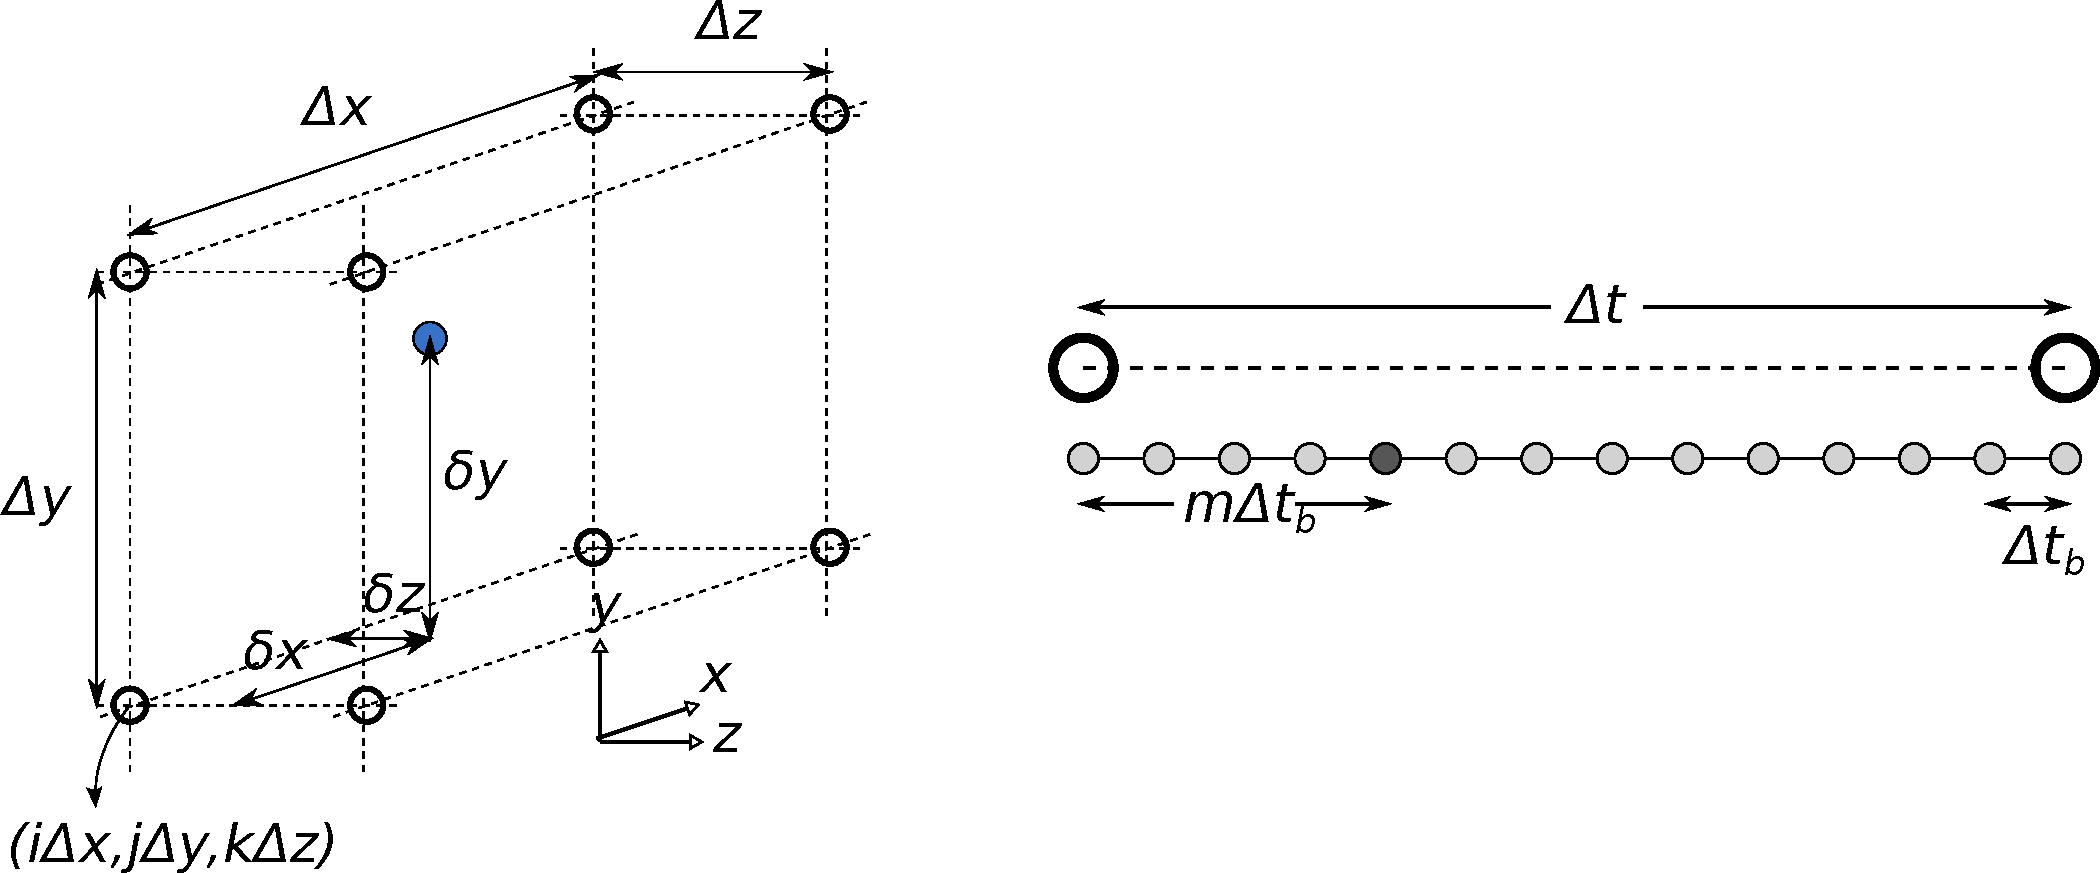
\includegraphics[height=2.0in]{./MITHRA_FDTDPIC/Fig1/Fig1.pdf}
\caption{Schematic illustration of the parameters used to locate a particle within the computational domain.}
\label{FDTDPICFig1}
\end{figure}
%
First, the values of magnetic and scalar potentials at $t+\Delta t/2$ are used to evaluate the electromagnetic fields at the cell vertices.
%
Subsequently, the field values are interpolated to the particle location for updating the equation of motion.
%
An important consideration at this stage is compatible interpolation of fields from the cell vertices with the interpolations used for current and charge densities.
%
Similar interpolation algorithms should be followed to cancel the effect of self-forces on particle motion.

Using the equation (\ref{BvsA}), the magnetic field $\vec{B}^n_{i,j,k}$ at cell vertex $(i,j,k)$ is calculated as follows:
%%
\begin{align}
{B_x}^n_{i,j,k} = & \frac{1}{2} \left( \frac{{A_z}_{i,j+1,k}^n-{A_z}_{i,j-1,k}^n}{2\Delta y} - \frac{{A_y}_{i,j,k+1}^n-{A_y}_{i,j,k-1}^n}{2\Delta z} + \frac{{A_z}_{i,j+1,k}^{n+1}-{A_z}_{i,j-1,k}^{n+1}}{2\Delta y} - \frac{{A_y}_{i,j,k+1}^{n+1}-{A_y}_{i,j,k-1}^{n+1}}{2\Delta z} \right), \\
{B_y}^n_{i,j,k} = & \frac{1}{2} \left( \frac{{A_x}_{i,j,k+1}^n-{A_x}_{i,j,k-1}^n}{2\Delta z} - \frac{{A_z}_{i+1,j,k}^n-{A_z}_{i-1,j,k}^n}{2\Delta x} + \frac{{A_x}_{i,j,k+1}^{n+1}-{A_x}_{i,j,k-1}^{n+1}}{2\Delta z} - \frac{{A_z}_{i+1,j,k}^{n+1}-{A_z}_{i-1,j,k}^{n+1}}{2\Delta x} \right), \\
{B_z}^n_{i,j,k} = & \frac{1}{2} \left( \frac{{A_y}_{i+1,j,k}^n-{A_y}_{i-1,j,k}^n}{2\Delta x} - \frac{{A_x}_{i,j+1,k}^n-{A_x}_{i,j-1,k}^n}{2\Delta y} + \frac{{A_y}_{i+1,j,k}^{n+1}-{A_x}_{i-1,j,k}^{n+1}}{2\Delta x} - \frac{{A_x}_{i,j+1,k}^{n+1}-{A_x}_{i,j-1,k}^{n+1}}{2\Delta y} \right).
\end{align}
%
Similarly, equation (\ref{EvsA}) is employed to evaluate the electric field at the cell vertices.
%
The electric field $\vec{E}^n_{i,j,k}$ is obtained from the following equations:
%
\begin{align}
{E_x}^n_{i,j,k} = & \left( -\frac{{A_x}_{i,j,k}^{n+1}-{A_x}_{i,j,k}^n}{\Delta t} - \frac{\varphi_{i+1,j,k}^n-\varphi_{i-1,j,k}^n}{2\Delta x} \right), \\
{E_y}^n_{i,j,k} = & \left( -\frac{{A_y}_{i,j,k}^{n+1}-{A_y}_{i,j,k}^n}{\Delta t} - \frac{\varphi_{i,j+1,k}^n-\varphi_{i,j-1,k}^n}{2\Delta y} \right), \\
{E_z}^n_{i,j,k} = & \left( -\frac{{A_z}_{i,j,k}^{n+1}-{A_z}_{i,j,k}^n}{\Delta t} - \frac{\varphi_{i,j,k+1}^n-\varphi_{i,j,k-1}^n}{2\Delta z} \right).
\end{align}

Suppose that a particle resides at the cell $ijk$ with the grid point indices shown in Fig.\,\ref{FDTDPICFig1}. %
%
As illustrated in Fig.\ref{FDTDPICFig1}, the distance to the corner $(i\Delta x, j\Delta y, k \Delta z)$ is assumed to be $(\delta x, \delta y, \delta z)$.
%
We use a linear interpolation of the fields from the vertices to the particle position to calculate the imposed field.
%
If $\varsigma$ denotes for a component of the electric or magnetic field, i.e. $\varsigma \in \{ E_x, E_y, E_z, B_x, B_y, B_z \}$, one can write
%
\begin{equation}
\label{fieldInterpolation}
\varsigma^p = \sum\limits_{I,J,K} \left(\frac{1}{2} + (-1)^I \left| \frac{1}{2} - \frac{\delta x}{\Delta x} \right| \right)
\left(\frac{1}{2} + (-1)^J \left| \frac{1}{2} - \frac{\delta y}{\Delta y} \right| \right)
\left(\frac{1}{2} + (-1)^K \left| \frac{1}{2} - \frac{\delta z}{\Delta z} \right| \right) \varsigma_{i+I,j+J,k+K},
\end{equation}
%
where $I$, $J$, and $K$ are equal to either 0 or 1, producing the eight indices corresponding to the eight corners of the mesh cell.

\subsection{Current Deposition}

Once the position and momentum of all the particles over the time interval $\Delta t $ is known, one needs to couple the pertinent currents into the wave equation (\ref{WaveA}).
%
As described before, this coupling over time is implemented through the equation (\ref{currentIntegral}).
%
The remaining question is how to evaluate the related currents on the grid points, i.e. the method for performing an spatial interpolation.
%
To maintain consistency, we should use a similar interpolation scheme as used for the field evaluation.
%
This assumption leads to the following equation for spatial interpolation.
%
\begin{equation}
{\rho^p}_{i+I,j+J,k+K} = \rho \left(\frac{1}{2} + (-1)^I \left| \frac{1}{2} - \frac{\delta x}{\Delta x} \right| \right)
\left(\frac{1}{2} + (-1)^J \left| \frac{1}{2} - \frac{\delta y}{\Delta y} \right| \right)
\left(\frac{1}{2} + (-1)^K \left| \frac{1}{2} - \frac{\delta z}{\Delta z} \right| \right)
\end{equation}
%
where $\rho$ is the charge density attributed to each macro-particle, namely $q/(\Delta x \Delta y \Delta z)$.
%
${\rho^p}_{i,j,k}$ is the charge density at the grid point $(i,j,k)$ due to the moving particle $p$ in the computational mesh cell (Fig.\,\ref{FDTDPICFig1}a).
%
$I$, $J$, and $K$ are equal to either 0 or 1, which produce the eight indices corresponding to the eight corners of the mesh cell.
%
The total charge density $\rho_{i,j,k}$ will be a superposition of all the charge densities due to the moving particles of the bunch.
%
We have removed the superscripts corresponding to the time instant, to avoid the confusion due to different time marching steps $\Delta t$ and $\Delta t_b$.
%
The above interpolation is carried out at each update step of the field values.
%
One can consider the above interpolation equations as a rooftop charge distribution centered at the particle position and expanding in the regions $(-\Delta x < x < \Delta x, -\Delta y < y < \Delta y, -\Delta z < z < \Delta z)$.
%
Eventually, the equation (\ref{currentIntegral}) is used to calculate the corresponding current densities.

The combination of equation (\ref{currentIntegral}) and (\ref{chargeIntegral}) should maintain the charge conservation law (equation (\ref{chargeLaw})) in a discretized space.
%
For this purpose, the projection from position vectors $\vec{r}$ to the Cartesian components in (\ref{currentIntegral}) should be done using the so-called ZigZag scheme proposed in \cite{umeda2003new}.
%
According to this scheme when a particle moves from the point $(x_1,y_1,z_1)$ to $(x_2,y_2,z_2)$, the motion is divided into two separate movements, namely (i) from $(x_1,y_1,z_1)$ to $(x_r,y_r,z_r)$, and (ii) from $(x_r,y_r,z_r)$ to $(x_2,y_2,z_2)$.
%
The coordinates of the relay point $(x_r,y_r,z_r)$ are obtained from the following equation:
%
\begin{align}
x_r = \min\left[ \min(i_1 \Delta x,i_2 \Delta x) + \Delta x, \nonumber \max\left( \max(i_1 \Delta x,i_2 \Delta x), \frac{x_1+x_2}{2} \right) \right] \nonumber \\
y_r = \min\left[ \min(j_1 \Delta y,j_2 \Delta y) + \Delta y, \nonumber \max\left( \max(j_1 \Delta y,j_2 \Delta y), \frac{y_1+y_2}{2} \right) \right] \\
z_r = \min\left[ \min(k_1 \Delta z,k_2 \Delta z) + \Delta z, \nonumber \max\left( \max(k_1 \Delta z,k_2 \Delta z), \frac{z_1+z_2}{2} \right) \right] \nonumber
\end{align}
%
where $(i,j,k)$ with indices 1 and 2 represent the cell numbers containing the initial and final points, respectively.
%
Since potential $\vec{A}$ and $\varphi$ are obtained from current and charge in exactly similar ways (update equations), if charge and current obey the charge conservation, the gauge condition will be automatically satisfied.
%
In other words, if the initial potentials satisfy the gauge condition, solving equations (\ref{WaveA}), (\ref{WaveF}), and (\ref{chargeLaw}) results in potential distributions at time $t$ which also satisfy the gauge condition.
%
The only requirement is that both potentials are discretized and updated in the same way.

\section{Quantity Initialization}

The previous two sections on FDTD and PIC algorithms present a suitable and efficient framework for the computation of interaction between charged particles and propagating waves.
%
However, the initial conditions are always required for a complete determination of the problem of interest.
%
For a FEL simulation, the initial conditions corresponding to the FEL input are given to the FDTD/PIC solver.
%
For example, in case of a SASE (Self Amplified Spontaneous Emission) FEL, the initial fields are zero and there is no excitation entering the computational domain, whereas for a seeded FEL, an outside excitation should be considered entering the computational domain.
%
The explanation of how such initializations are implemented in MITHRA is the goal in this section.

One novel feature of the method, followed here, is the solution of Maxwell's equations in the bunch rest frame.
%
It can be shown that a proper coordinate transformation yields the matching of all the major parameters in a FEL simulation, namely bunch length, undulator period, undulator length, and radiation wavelength.
%
\begin{figure}
\centering
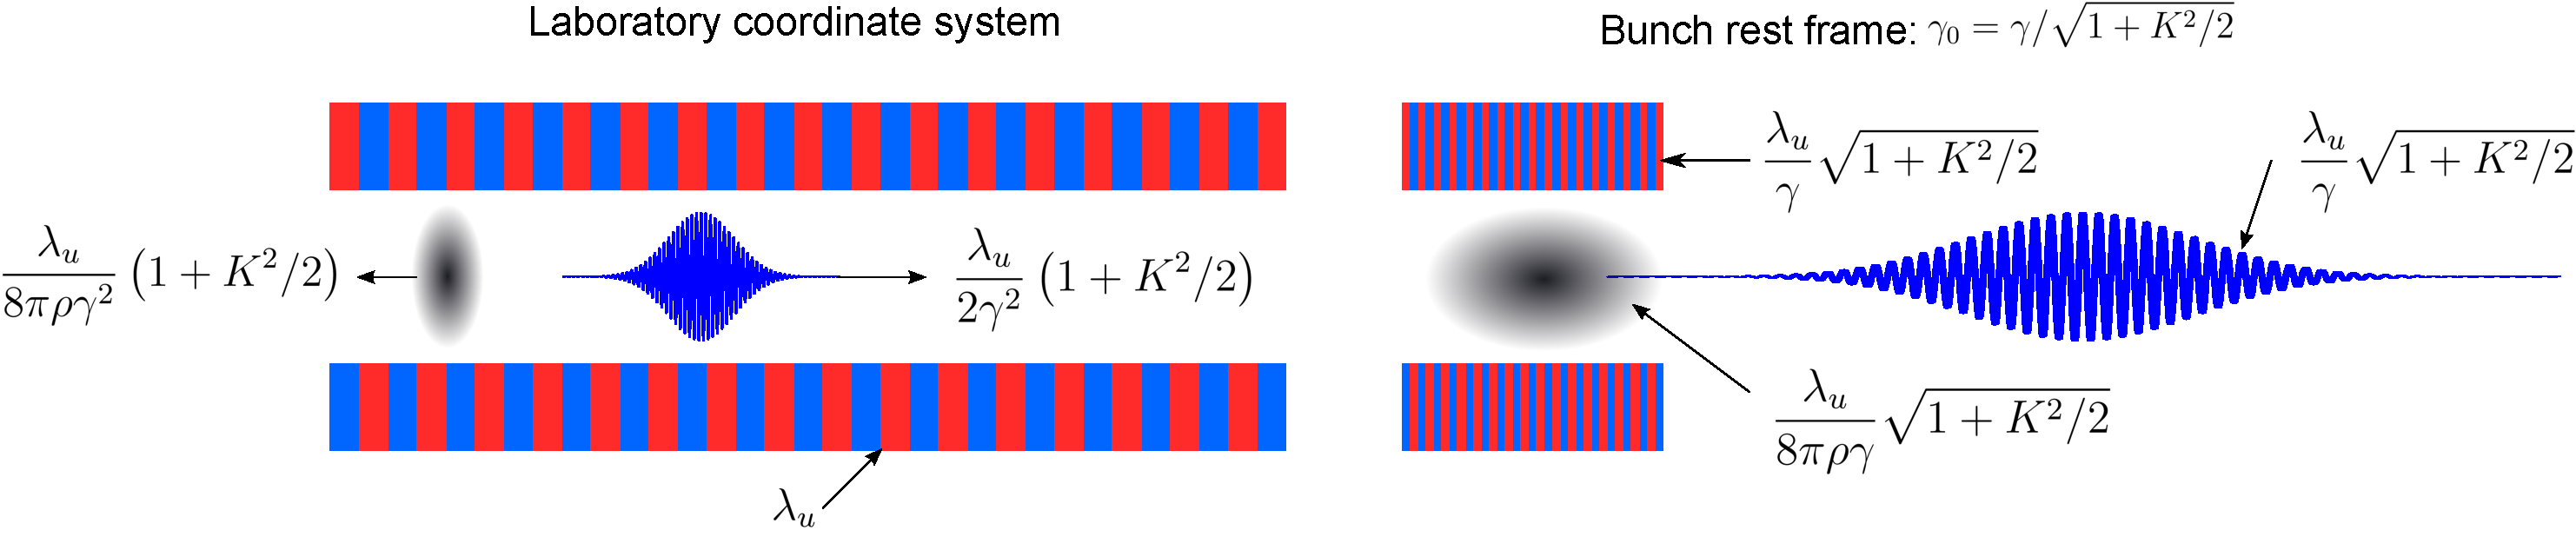
\includegraphics[width=7.0in]{./MITHRA_FDTDPIC/Fig2/Fig2.pdf}
\caption{Schematic illustration of the Lorentz boosting to transform the problem from the laboratory frame to the bunch rest frame.}
\label{FDTDPICFig2}
\end{figure}
%
Fig.\,\ref{FDTDPICFig2} schematically describes the advantage of moving into the bunch rest frame.
%
In a typical FEL problem, the FEL parameter $\rho_{FEL}$ is about $10^{-3}$.
%
Therefore, simulation of FEL interaction with a bunch equal to the cooperation length of the FEL ($L_c=\lambda_l/(4 \pi \rho_{FEL})$, with $\lambda_l$ being the radiation wavelength) requires a simulation domain only 100 times larger than the wavelength.
%
This becomes completely possible with the today computer technology and constitutes the main goal of MITHRA.
%
In this section, the main basis for Lorentz boosting the simulation coordinate is described first.
%
Afterwards, the relations for evaluating the undulator fields in the Lorentz boosted framework are presented.
%
Finally, the electron bunch initialization in the Lorentz-boosted framework is discussed.

\subsection{Lorentz Transformation}

It is known from the FEL thoery that a bunch with central Lorentz factor equal to $\gamma$ moves in an undulator with an average Lorentz factor equal to $\gamma_0=\gamma/\sqrt{(1+K^2/2)}$, where $K=eB\lambda_u/(2\pi m c)$ is the undulator parameter determining the amplitude of the wiggling motion.
%
Consequently, a frame moving with normalized velocity $\beta_0 = \sqrt{1-1/\gamma_0^2}$ is indeed the bunch rest frame, where the volume of the computational domain stays minimal.
%
Transforming into this coordinate system necessitates tailoring the bunch and undulator properties.
%
For this purpose, the Lorentz length contraction, time dilation and relativistic velocity addition need to be employed.

In MITHRA, the input parameters are all taken in the laboratory frame and the required Lorentz transformations are carried out based on the bunch energy.
%
The required transformations for the computational mesh are as the following:
%
\begin{align}
\Delta z & = \Delta z' \gamma_0,  \label{LorentzTransformB}\\
\Delta t & = \Delta t' / \gamma_0,  \\
\Delta t_b & = \Delta t'_b / \gamma_0,
\end{align}
%
where the prime sign stands for the quantities in the laboratory frame.
%
The quantities without prime are values in the bunch rest frame, which are used in the FDTD/PIC simulation.
%
With the consideration of the above transformations, the length of the total computational domain along the undulator period and the total simulation time is also transformed similarly.

In addition to the data for the computational mesh, the properties of the electron bunch also changes after the Lorentz boosting.
%
This certainly affects the bunch initialization process which is thoroughly explained in the next section.
%
An electron bunch in MITHRA is initialized and characterized by the following parameters:
%
\begin{enumerate}[(i)]
\item Mean electron position: $(\bar{x}_b, \bar{y}_b, \bar{z}_b)$,
\item Mean electron normalized momentum: $(\overline{\gamma \beta}_x, \overline{\gamma \beta}_y, \overline{\gamma \beta}_z)$,
\item RMS value of the electron position distribution: $(\sigma_x, \sigma_y, \sigma_z)$,
\item RMS value of the electron normalized momentum distribution: $(\sigma_{\gamma \beta_x}, \sigma_{\gamma \beta_y}, \sigma_{\gamma \beta_z})$.
\end{enumerate}
%
As mentioned previously, the above parameters are entered by the user in the laboratory frame.
%
To transform the given values to the bunch rest frame the position related parameters are changed as
%
\begin{equation}
\begin{array}{cccccc}
\bar{x}_b = \bar{x}'_b, & \bar{y}_b = \bar{y}'_b, & \bar{z}_b = \displaystyle \frac{\bar{z}'_b}{\gamma_0 (1 - \bar{\beta'}_z \beta_0)} , & \sigma_x = \sigma'_x, & \sigma_y = \sigma'_y, & \sigma_z = \displaystyle \frac{\sigma'_z}{{\gamma_0 (1 - \bar{\beta'}_z \beta_0)}}.
\end{array}
\end{equation}
%
To transfer the momentum related quantities, we assume that the main contribution to the Lorentz factor is the momentum along $z$ direction or the undulator period.
%
In other words, $(\overline{\gamma \beta}_x, \overline{\gamma \beta}_y, \overline{\gamma \beta}_z) = \gamma ( \bar{\beta}_x, \bar{\beta}_y, \bar{\beta}_z )$, with $\gamma = 1/\sqrt{1-\bar{\beta}_z^2}$.
%
Similarly, the RMS values can also be written as $(\sigma_{\gamma \beta_x}, \sigma_{\gamma \beta_y}, \sigma_{\gamma \beta_z}) = \gamma (\sigma_{\beta_x}, \sigma_{\beta_y}, \sigma_{\beta_z})$.
%
Using the relativistic velocity transformation \cite{JacksonClassical}, the transformation equations for the above values are found as follows:
%
\begin{align}
\gamma & = \gamma' \gamma_0 (1 - \bar{\beta'}_z \beta_0), \\
( \bar{\beta}_x, \bar{\beta}_y, \bar{\beta}_z ) & = ( \bar{\beta'}_x, \bar{\beta'}_y, \sqrt{1 - 1/\gamma^2} ), \\
(\sigma_{\gamma \beta_x}, \sigma_{\gamma \beta_y}, \sigma_{\gamma \beta_z}) & = (\sigma'_{\gamma \beta_x}, \sigma'_{\gamma \beta_y}, \sigma'_{\gamma \beta_z} ) \gamma_0 (1 - \bar{\beta'}_z \beta_0). \label{LorentzTransformE}
\end{align}
%
Equations (\ref{LorentzTransformB})-(\ref{LorentzTransformE}) provide a sufficient set of equations to perform the Lorentz boost to the bunch rest frame.

\subsection{Field Initialization}
\label{fieldInitialization}

The utilized FDTD/PIC algorithm solves the Maxwell's equation coupled with the motion equation of an ensemble of particles.
%
Therefore, in addition to the field values, particle initial conditions should also be initialized.
%
For a SASE FEL problem, the initial field profile is zero everywhere, whereas for a seeded FEL the initial seed should enter the computational domain through the boundaries.
%
In both cases, the external field which is the undulator field should separately be initialized.
%
In what follows, the equations implemented in the code for initializing the undulator fields and seed fields are explained.

\subsubsection{Static Undulator Field:}

By solving the Laplace equation for the magnetic field, the undulator field in the laboratory frame is found to be as the following (Fig.\,\ref{FDTDPICFig3}) \cite{FEL2}:
%
\begin{figure}
\centering
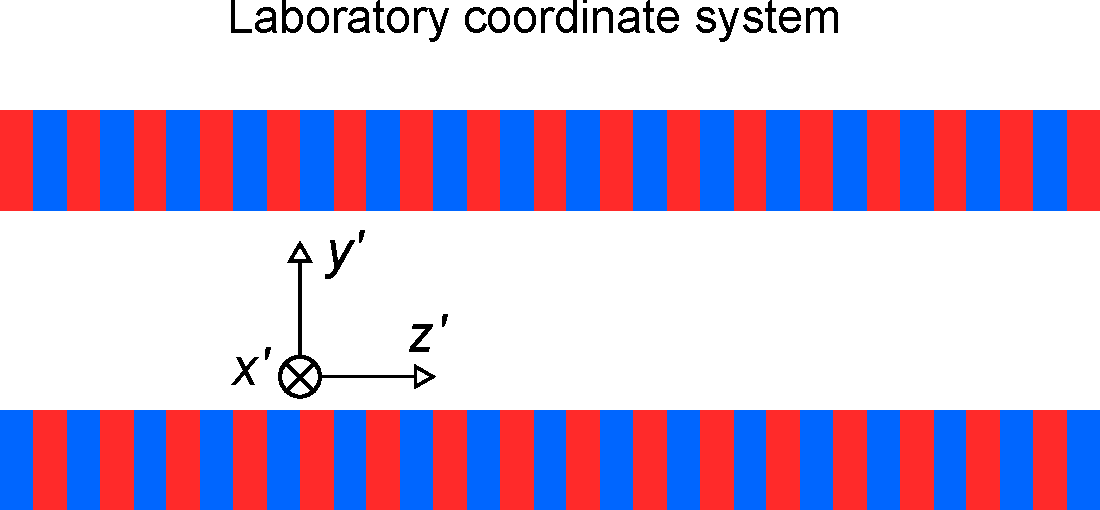
\includegraphics[width=3.2in]{./MITHRA_FDTDPIC/Fig3/Fig3.pdf}
\caption{Schematic illustration of the undulator in the lab frame and the definition of the coordinates.}
\label{FDTDPICFig3}
\end{figure}
%
\begin{align}
\label{undulatorField}
B'_x & = 0, \nonumber \\
B'_y & = B_0 \cosh(k_uy')\sin(k_uz'), \\
B'_z & = B_0 \sinh(k_uy')\cos(k_uz'), \nonumber
\end{align}
%
where $B_0$ is the maximum transverse field of the undulator.
%
To calculate the undulator field in the bunch rest frame, first the position is transformed to laboratory frame $(x',y',z')$ through the Lorentz boost equations.
%
Afterwards, the field is evaluated using the equation (\ref{undulatorField}).
%
Ultimately, these fields are transformed back into the bunch rest frame.
%
The above approach, although adds few mathematical operations for the calculation of undulator fields, it enables straightforward implementation of various realistic effects, like fringing fields of the entrance section and non-gaussian field profiles.

An important consideration in the initialization of undulator field is the entrance region of the undulator.
%
A direct usage of the equation (\ref{undulatorField}) with zero field for $z'<0$ causes an abrupt variation in the particles motion, which results in a spurious coherent radiation.
%
In fact, in a real undulator, there exists fringing fields at the undulator entrance, which remove any abrupt transition in the undulator field and consequently the particle radiations  \cite{sagan2003magnetic}.
%
To the best of our knowledge, the fringing fields are always modeled numerically and there exists no analytical solution for the problem.
%
Here, we approximate the fringing fields by a gradually decreasing magnetic field in form of a Neumann function.
%
The coefficients in the function are set such that the particles do not gain any net transverse momentum and stay in the computational domain as presumed.
%
The undulator field for $z'<0$ in the laboratory frame is obtained as the following:
%
\begin{align}
B'_x & = 0, \nonumber \\
B'_y & = B_0 \cosh(k_uy')k_uz'e^{-(k_uz')^2/2}, \label{fringingField} \\
B'_z & = B_0 \sinh(k_uy')e^{-(k_uz')^2/2}, \nonumber
\end{align}

Equations (\ref{undulatorField}) and (\ref{fringingField}) return the fields in the stationary frame of the undulator, i.e. the laboratory frame.
%
To obtain the fields in the bunch rest frame, MITHRA first transfers the coordinate of input bunch from rest frame to the laboratory frame using Lorentz coordinate transformations:
%
\begin{align}
x' & = x, \nonumber \\
y' & = y, \label{LorentzTransformR2L} \\
z' & = \gamma_0(z+\beta_0ct), \nonumber
\end{align}
%
Then, the undulator field is calculated at point $(x',y',z')$ using (\ref{undulatorField}) and (\ref{fringingField}).
%
Afterwards, the calculated field is transferred back to the bunch rest frame using the Lorentz transformation for the electromagnetic fields:
%
\begin{align}
\label{LorentzTransformElectric}
\vec{E} & = \gamma_0 (\vec{E'}+c\vec{\beta_0} \times \vec{B'}) - (\gamma_0 - 1) E'_z \hat{\vec{z}}, \\
\label{LorentzTransformMagnetic}
\vec{B} & = \gamma_0 (\vec{B'}-\frac{\vec{\beta_0} \times \vec{E'}}{c^2}) - (\gamma_0 - 1) B'_z \hat{\vec{z}},
\end{align}
%
where $\vec{\beta_0}=\beta_0\hat{\vec{z}}$. Since the undulator field in the lab frame is purely magnetic, in the above equation $\vec{E'}=0$.

\subsubsection{Static Undulator Array Field:}

Calculating the field of an undulator array is identical to the field of a single module, except for the gap region between the undulator modules.
%
If the equation (\ref{fringingField}) is used for each module, and simply superposed at the gap, the field values close to the two undulator boundaries will be overestimated.
%
To solve this problem, suitable functions should on one side resemble the Gaussian damping of the field and on the other side vanish at the other end of the gap.
%
In MITHRA, the following field variation is assumed for the fringing fields inside the gap:
%
\begin{align}
B'_x & = 0, \nonumber \\
B'_y & = B_0 \cosh(k_uy')k_u\delta z e^{-(k_u \delta z)^2/2} f(\delta z,g), \label{fringingFieldGap} \\
B'_z & = B_0 \sinh(k_uy') e^{-(k_u \delta z)^2/2} f(\delta z,g), \nonumber
\end{align}
%
with
%
\begin{equation}
f(\delta z, g) = 0.35875 + 0.48829 \cos( \frac{\pi \delta z}{g} ) + 0.14128 \cos( \frac{2 \pi \delta z}{g} ) + 0.01168 \cos( \frac{3 \pi \delta z}{g} )
\end{equation}
%
where $\delta z$ is the distance to the undulator entrance and $g$ is the gap length between the two undulators.
%
Note that both equations (\ref{fringingField}) and (\ref{fringingFieldGap}) are approximations of the field damping at the end of the undulator.
%
An accurate formulation is not possible since there exists no analytical solution for the fringing fields.
%
In order to better figure out the field variations in the gap region, the transverse magnetic field ($B'_y$) on the undulator axis inside an undulator and an undulator array are compared with each other in Fig.\,\ref{FDTDPICFig4}.
%
\begin{figure}
	\centering
	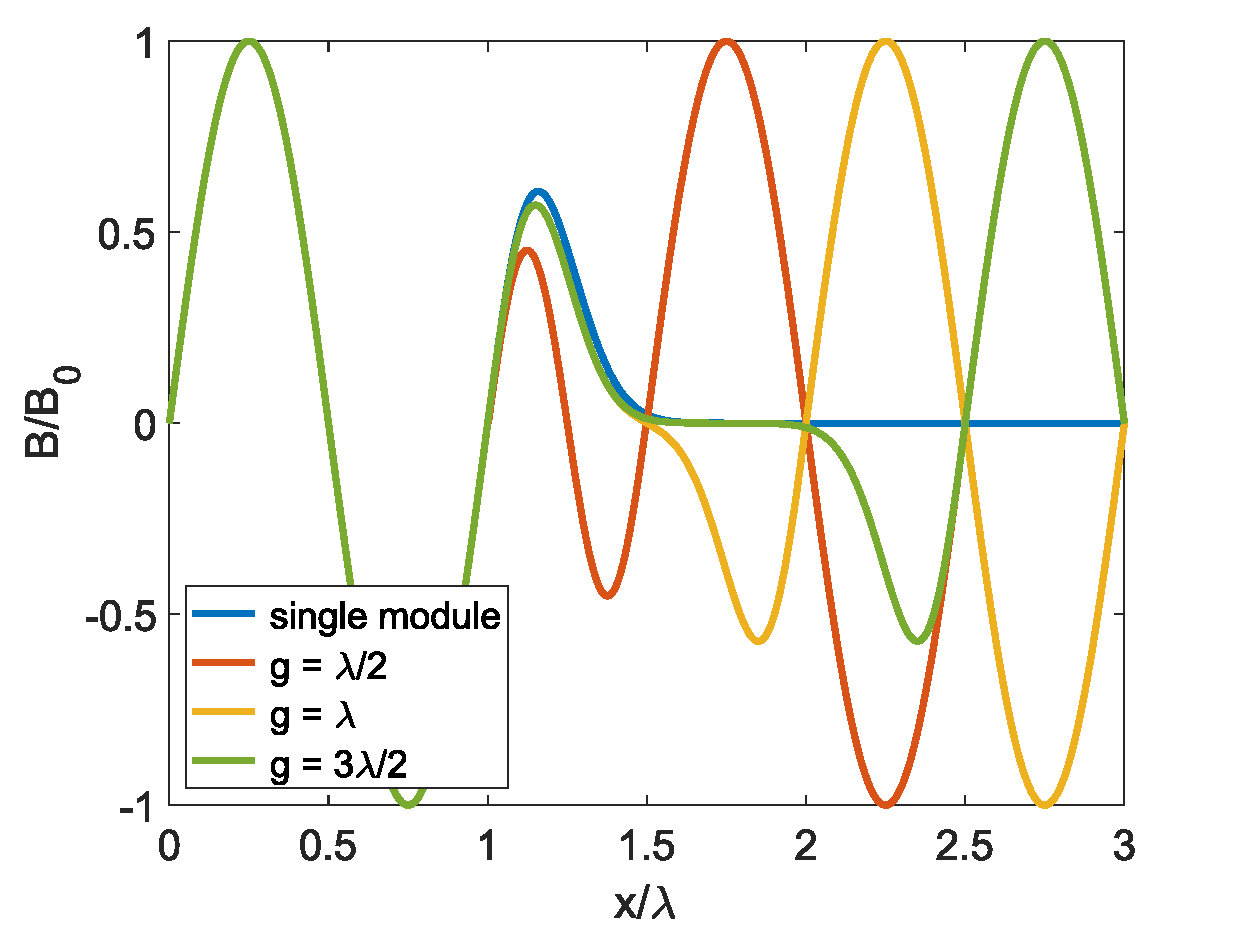
\includegraphics[width=3.4in]{./MITHRA_FDTDPIC/Fig4/Fig4.pdf}
	\caption{Normalized magnetic field at the center of undulator within the undulator and in the fringing field regions. Four cases are visualized and compared: (i) a single undulator module, and two undulator modules with a gap equal to (ii) half the wavelength, (ii) one wavelength, and (iii) one and a half wavelength}
	\label{FDTDPICFig4}
\end{figure}

\subsubsection{Optical Undulator Field:}

The wiggling motion of electrons required for radiation generation can also be instigated by the oscillating fields of an electromagnetic wave.
%
This is the main idea behind another undulator type named as optical undulator.
%
These undulators are typically in form of an electromagnetic beam propagating counter to the electron beam.
%
If the beam is a plane-wave, the fields are obtained as follows:
%
\begin{align}
\label{opticalUndulatorPW}
E_\parallel & = E_0 f(t,t_0,\phi) , \nonumber \\
B_\bot & = \frac{E_0}{c} f(t,t_0,\phi), \\
E_\bot & = B_\parallel = E_l = B_l = 0, \nonumber
\end{align}
%
where $\bot$ and $\parallel$ indices represent field values perpendicular and parallel to the polarization direction respectively.
%
Subscript $l$ denotes the longitudinal direction along the propagation line, which can be different from the undulator axis $z$.
%
$f(t,t_0,\phi)$, with $t_0$ being the time offset and $\phi$ the carrier-envelope phase (CEP), is the time signature of the incoming pulse.
%
Various signatures are implemented in MITHRA, which are listed in equation (\ref{signalTypes}).

A more practical assumption for the counter-propagating beam is a Gaussian beam.
%
The fields of a Gaussian beam is obtained from
%
\begin{align}
\label{opticalUndulatorGB}
& E_\parallel = E_0 \sqrt{\frac{w_{0\parallel}w_{0\bot}}{w_\parallel (l)w_\bot (l)}} 
\exp\left( -\frac{r_\bot^2}{w_\bot^2}-\frac{r_\parallel^2}{w_\parallel^2} \right) 
f\left(t,t_0,-\frac{k_0 r_\parallel^2}{2R_\parallel(l)} - \frac{k_0 r_\bot^2}{2R_\bot(l)} - \frac{\pi}{2} + \frac{ \tan^{-1} \left(\frac{l}{z_{R\parallel}}\right) + \tan^{-1} \left(\frac{l}{z_{R\bot}} \right) }{2} \right), \nonumber \\
& E_l = E_0 \frac{r_\parallel w_{0\parallel}}{z_{R\parallel} w_\parallel(l)} \sqrt{\frac{w_{0\parallel}w_{0\bot}}{w_\parallel(l)w_\bot (l)}} 
\exp\left( -\frac{r_\bot^2}{w_\bot^2}-\frac{r_\parallel^2}{w_\parallel^2} \right) 
f\left(t,t_0,-\frac{k_0 r_\parallel^2}{2R_\parallel(l)} - \frac{k_0 r_\bot^2}{2R_\bot(l)} + \frac{ 3\tan^{-1} \left(\frac{l}{z_{R\parallel}}\right) + \tan^{-1} \left(\frac{l}{z_{R\bot}} \right) }{2} \right), \nonumber \\
& B_l = \frac{E_0 r_\bot w_{0\bot}}{c z_{R\bot} w_\bot(l)} \sqrt{\frac{w_{0\parallel}w_{0\bot}}{w_\parallel (l)w_\bot (l)}} 
\exp\left( -\frac{r_\bot^2}{w_\bot^2}-\frac{r_\parallel^2}{w_\parallel^2} \right) 
f\left(t,t_0,-\frac{k_0 r_\parallel^2}{2R_\parallel(l)} - \frac{k_0 r_\bot^2}{2R_\bot(l)} + \frac{ \tan^{-1} \left(\frac{l}{z_{R\parallel}}\right) + 3 \tan^{-1} \left(\frac{l}{z_{R\bot}} \right) }{2} \right), \nonumber \\
& B_\bot = \frac{E_\parallel}{c}, \qquad E_\parallel = B_\bot = 0
\end{align}
%
where $\bot$ and $\parallel$ indices represent field components normal to the propagation direction, perpendicular and parallel to the polarization vector, respectively.
%
$l$, as a subscript for the fields, stands for the component along propagation direction, and as a variable is the position along this direction, i.e. $r_l$.
%
$w_\parallel=w_{0\parallel}\sqrt{1+(r_\parallel/z_{R\parallel})^2}$ and $w_\bot=w_{0\bot}\sqrt{1+(r_\bot/z_{R\bot})^2}$ with $w_{0\parallel}$ being the beam radius along the polarization vector, $w_{0\bot}$ the beam radius normal to the polarization vector, and $z_{R\parallel}$ and $z_{R\bot}$ are the corresponding Rayleigh range values.
%
Parameters $R_\parallel(l)=l(1+(z_{R\parallel}/l)^2)$ and $R_\bot(l)=l(1+(z_{R\bot}/l)^2)$ are defined as radius of the curvature of the beam's wavefronts at position $l$.

\subsubsection{Seed Field:}

External excitation of free electron laser process using a seed mechanism has proved to be advantageous in terms of output spectrum, photon flux and the required undulator length  \cite{pellegrini2016physics,FEL2}.
%
Such benefits has propelled the proposal of seeded FEL schemes.
%
To simulate such a mechanism, MITHRA uses the TF/SF (total-field/scattered-field) technique to introduce an external excitation into the computational domain.
%
When seeding is enabled by having a non-zero seed amplitude, the second and third points (after the boundary points) constitute the scattered and total field boundaries, respectively.
%
Therefore, during the time marching process, after each update according to equation (\ref{updateEquation}) the excitation terms are added to the fields at TF/SF boundaries.
%
For example for the TF/SF boundaries close to $z=z_{min}$ plane, the field values to be used in the next time steps are obtained as the following:
%
\begin{align}
\text{ SF boundary:  } & \psi_{i,j,k}^{'n+1} = \psi_{i,j,k}^{n+1} + \mathcal{A} ( \alpha'_2 f_{i+1,j,k+1}^n  + \alpha'_3 f_{i-1,j,k+1}^n + \alpha'_4 f_{i,j+1,k+1}^n + \alpha'_5 f_{i,j-1,k+1}^n ) + \alpha'_6 f_{i,j,k+1}^n, \nonumber \\
\text{ TF boundary:  } & \psi_{i,j,k}^{'n+1} = \psi_{i,j,k}^{n+1} - \mathcal{A} ( \alpha'_2 f_{i+1,j,k-1}^n  + \alpha'_3 f_{i-1,j,k-1}^n + \alpha'_4 f_{i,j+1,k-1}^n + \alpha'_5 f_{i,j-1,k-1}^n ) - \alpha'_7 f_{i,j,k-1}^n,
\end{align}
%
where $f_{i,j,k}^n$ is the excitation value at time $n\Delta t$ and position $(i\Delta x,j\Delta y,k\Delta z)$.
%
The excitation value is calculated based on the imposed seed fields, which are usually either a plane wave or a Gaussian beam radiation.

\subsection{Electron Bunch Generation}

\subsubsection{Position and momentum initialization:}

As described previously, the evolution of the electron bunch is always simulated by following the macro-particle approach, where an ensemble of particles are represented by one sample particle.
%
This typically reduces the amount of computation cost for updating the bunch properties by three or four orders of magnitude.
%
Due to the high sensitivity of a FEL problem to the initial conditions, correct and proper initialization of these macro-particles play a critical role in obtaining reliable results.
%
In computational accelerator physics, different approaches are introduced and developed for bunch generation.
%
Some examples are random generation of particles, mirroring macro-particles at different phases to prevent initial average bunching factors, and independent random filling of different coordinates to prevent unrealistic correlations \cite{reiche2000numerical}.
%
Among all the different methods, using the sophisticated methods to load the bunch in a "quasi-random" manner seem to be the most appropriate solutions.
%
The Halton or Hammersley sequences, as generalizations of the bit-reverse techniques, are implemented in MITHRA for particle generation.
%
These sequences compared to random based filling of the phase space avoid the appearance of local clusters in the bunch distribution.

Moreover, such a uniform filling of the phase space prevents initial bunching factor of the generated electron bunch.
%
This aspect is very beneficial in FEL simulations, since it removes any spurious initial radiation.
%
Subsequently, the initial bunching factor or shot noise can be manually added to the particle distribution in a controlled fashion. 
%
For details on the nature of Halton sequences, the reader is referred to the specialized documents.
%
Here, we only present the implemented algorithm to generate the required sequence of numbers filling the interval $[0,1]$.
%
The following C++ function is integrated into MITHRA which produces $N<20$ uncorrelated sequences including arbitrary number of elements in the interval $[0,1]$:
%
\begin{multicols}{2}
	\setlength{\columnseprule}{0.2pt}
	\begin{Verbatim}[fontsize=\footnotesize, tabsize=2, fontfamily=courier,	fontseries=b]
	Double halton (unsigned int i, unsigned int j)
	{
		unsigned int prime [20] = {2, 3, 5, 7, 11, 13, 
			 17, 19, 23, 29, 31, 37, 41, 43, 47, 53, 59, 
			 61, 67, 71};
		int p0, p, k, k0, a;
		Double x = 0.0;
	
		k0 = j;
	
		p = prime[i];
	
		p0 = p;
		k  = k0;
		x  = 0.0;
		while (k > 0)
			{
				a   = k % p;
				x  += a / (double) p0;
				k   = int (k/p);
				p0 *= p;
			}
	
		return 1.0 - x;
	}
	\end{Verbatim}
\end{multicols}
%
\noindent By having the above uniform distributions, the 6D phase space of the initial bunch can be filled according to the desired bunch properties.

In MITHRA, different schemes for the user is implemented to generate the initial electron bunch, which are described in chapter \ref{chapter_refcard}.
%
The main requirements for initializing the bunches is to generate 1D and 2D set of numbers with either uniform or Gaussian distributions.
%
Suppose $x_1$ and $x_2$ are two uncorrelated number sequences produced by the Halton algorithm.
%
A 1D uniform distribution $y_1$ with average $y_{m1}$ and total width $y_{s1}$ is found by the following transformation:
%
\begin{equation}
\label{uniform1D}
y_1 = y_{s1} (x_1 - \frac{1}{2}) + y_{m1}.
\end{equation}
%
Such a distribution is used when a bunch with uniform current profile ($z$ distribution of particles) is to be initialized.
%
On the other hand, a 1D Gaussian distribution is needed when radiation of a bunch with Gaussian current profile is modelled.
%
To generate bunches with Gaussian distribution, we employ Box-muller's theory to extract a sequence of numbers with Gaussian distribution from two uncorrelated uniform distributions.
%
Based on this theory, a 1D Gaussian distribution $y_2$ with average $y_{m2}$ and deviation width $y_{s2}$ is found by the following transformation:
%
\begin{equation}
\label{gaussian1D}
y_2 = y_{s2} \sqrt{-2 \ln x_1} \cos(2\pi x_2) + y_{m2}.
\end{equation}

Similar to the undulator fields, an abrupt variation in the bunch profile results in an unrealistic coherent scattering emission (CSE), which happens if the uniform bunch distribution is directly initialized from equation (\ref{uniform1D}).
%
CSE is avoided by imposing smooth variations in the particle distribution.
%
For this purpose, we follow the procedure proposed in \cite{penman199282} and \cite{reiche2000numerical}.
%
A small Gaussian bunch with the same density as the real bunch and a width equal to an undulator wavelength is produced.
%
The lower half of the bunch (particles with smaller $z$) is transferred to the tail and the other half is placed at the head of the uniform bunch.
%
Hence, a uniform current profile with smooth variations at its head and tail is created.

The transverse coordinates of the bunches are initialized using 2D distributions.
%
In MITHRA, a 2D Gaussian distribution is assumed for transverse coordinates.
%
To generate such a distribution, two independent sets of numbers $x_1$ and $x_2$ are generated based on Halton sequence.
%
The desired 2D Gaussian distribution with average position $(y_{m3},y_{m4})$ and total deviation $(y_{s3},y_{s4})$ is produced as the following: %%
%
\begin{equation}
\label{gaussian2D}
\displaystyle y_3 = y_{s3} \sqrt{-2 \ln x_1} \cos(2\pi x_2) + y_{m3}, \qquad \mathrm{and} \qquad
\displaystyle y_4 = y_{s4} \sqrt{-2 \ln x_1} \sin(2\pi x_2) + y_{m4}.
\end{equation}
%
Such algorithms are similarly used to generate the distribution in particle momenta.
%
The only difference is that for initializing a distribution in momentum merely Gaussian profiles are considered in transverse and longitudinal coordinates.
%
The method to introduce these bunch types are described in the next chapter.

\subsubsection{Bunching factor:}

Free electron laser radiation should start from a nonzero initial radiation.
%
This radiation can be in form of an initial seed field, initial modulation in the bunch, or the radiation from bunch shot noise.
%
The implementation of seeding through an external excitation using TF/SF boundaries was described in \ref{fieldInitialization}.
%
Here, we explain how an initial bunching factor, $B = <e^{jk_uz}>$, is introduced to the electron bunch profile.

For this purpose, the methodology introduced in \cite{penman1992simulation} is followed. 
%
A small variation $\delta z$ is applied to a particle distribution generated using the described formulations.
%
$\delta z$ for each particle is obtained from
%
\begin{equation}
\label{bunchingFactor}
\delta z = \xi \gamma_0 k_u b_f \sin (2 \xi \gamma_0 k_u z),
\end{equation}
%
where $b_f$ is the given bunching factor of the distribution, and $\xi=1+\bar{\beta}_z/\beta_0$ accounts for the change in the bunch longitudinal velocity after entering the undulator.
%
The introduced variation to the bunch coordinates, i.e. $z \rightarrow z+\delta z$, yields a bunch with all the given particle and momentum distributions and the desired bunching factor, $b_f$.

\subsubsection{Shot noise:}

The number of particles (electrons) in a bunch is limited.
%
As a result, the average of bunching factor magnitudes over the whole bunch ($|B|^2=1/N_e$) does not tend to zero, meaning that there exists an initial total radiation in form of a noise.
%
This radiation commonly referred to as \emph{shot noise} can also be a trigger for the free-electron lasing process.
%
Such a mechanism is the basis for Self-Amplified Spontaneous Emission of radiation (SASE) type of FELs.
%
To simulate shot noise, bunch initialization starts with a uniform particle distribution obtained from Halton and Hammersley series.
%
Afterwards, a small variation $\delta z$ is applied to the particle distribution.
%
$\delta z$ for a particle residing in slice $j$ is obtained from
%
\begin{equation}
\label{bunchingFactor}
\delta z = \xi \gamma_0 k_u b_{fj} \sin (2 \xi \gamma_0 k_u z + \phi_j),
\end{equation}
%
where $b_{fj}$ and $\phi_j$ are the bunching factor value and phase in the slice j.
%
The other parameters are defined in the same way as described in the bunching factor section.
%
The value of $b_{fj}$ for different slices is obtained from a negative exponential distribution according to
%
\begin{equation}
\label{negativeExponential}
b_{fj} = \frac{1}{\sqrt{N_e}} \sqrt{-2 \ln x_j},
\end{equation}
%
where $x_j$ is obtained from a uniform Halton sequence.
%
The value of $\phi_j$ as the bunching factor phase in various slices is calculated based on a uniform distribution (i.e. Halton sequence) over the interval $[0,\pi]$.tttt 

\section{Parallelization}

The large and demanding computation cost needed for the simulation of the FEL process even in the Lorentz boosted coordinate frame necessitates solving the problem on multiple processors to achieve reasonable computation times.
%
Therefore, efficient parallelization techniques should be implemented in the FDTD/PIC algorithm to develop an efficient software.
%
Traditionally, there are two widely used techniques to run a computation in parallel on several processors: (1) \textit{shared} memory, and (2) \textit{distributed} memory parallelization.
%
In the shared memory parallelization or the so-called multi-threading technique, several processors run a code using the variables saved in one shared memory.
%
This technique is very suitable for PIC algorithms because it avoids the additional costs of communicating the particle position and momenta between the processors.
%
On the other hand, distributed memory technique distributes the involved variables among several processors, solves the problem in each processor independently and communicates the required variables whenever they are called.
%
The distributed memory technique is very suitable for FDTD algorithm due to the ease of problem decomposition beyond various machines.
%
The advantage is fast reading and writing of the data and the possibility to share the computational load between different machines.

Choosing a suitable parallelization scheme for the hybrid FDTD/PIC algorithm depends on both problem size and machine implementations.
%
In MITHRA, we use distributed memory technique for parallelization of the radiation computations.
%
The total computational domain is decomposed to several separate regions, each of them solved by one processor.
%
These sets of processors communicate the required variables based on the technique visualized in Fig.\,\ref{FDTDPICFig5}.
%
\begin{figure}
\centering
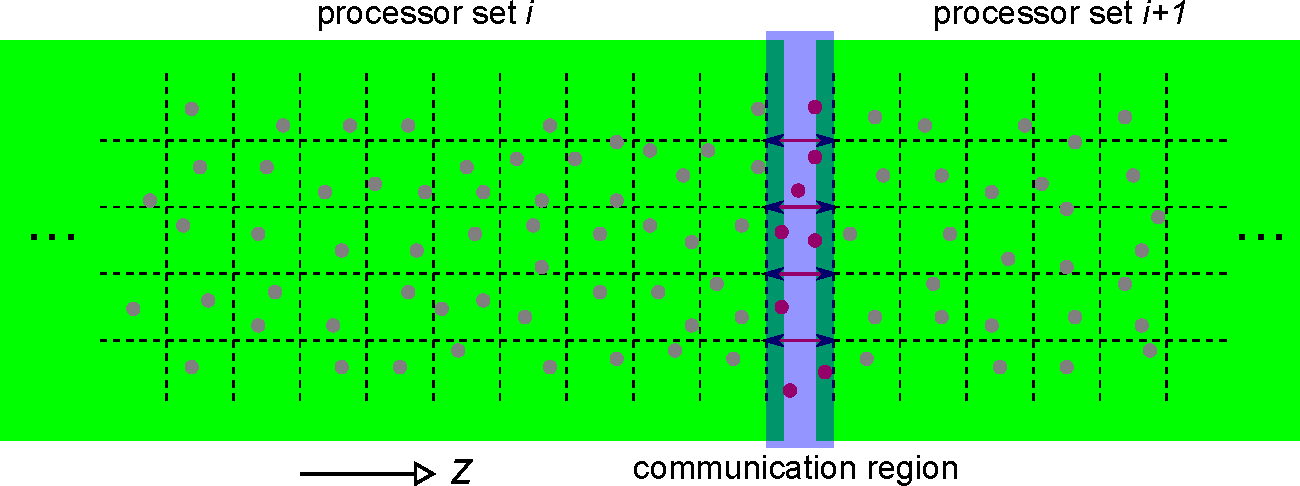
\includegraphics[width=5.0in]{./MITHRA_FDTDPIC/Fig5/Fig5.pdf}
\caption{Schematic illustration of the domain decomposition used for distributed memory parallelization in MITHRA}
\label{FDTDPICFig5}
\end{figure}

To parallelize the computation among $N$ processors, the whole computational domain is divided into $N$ domains along $z$ (undulator period) axis.
%
In each time update of the field, the field values at the boundaries of each domain are communicated with the corresponding processor.
%
To parallelize the PIC solver, we define a communication domain which as shown in Fig.\,\ref{FDTDPICFig5}, is the region between the boundaries of each processor.
%
After each update of the particles position, it is checked if the particle has entered a communication domain.
%
In case of residing in the communication region, the master processor, which is the processor containing the particle in the previous time step, communicates the new coordinates to the slave processor, which is the processor sharing the communication region with the master one.
%
Through this simple algorithm, the whole computation is distributed among the available processors of the machine. 